\chapter{INTRODUCTION}

\section{Background}

Partial discharge is defined as a localized dielectric breakdown of a small portion of a solid or fluid electrical insulation system under high voltage stress, which does not completely bridge the electrodes \parencite{Lu_2020_2}. It typically originates from insulation defects such as voids, cracks, surface contamination, or imperfections within high-voltage electrical equipment \parencite{Hussain_2021, Agarwal_2023}. These localized discharges degrade the insulation over time, potentially leading to insulation failure and catastrophic system breakdowns \parencite{Choudhary_2024_1}. Partial discharge plays a pivotal role as an early warning indicator in various high-voltage components including transformers, cable terminations, switchgear, and Gas Insulated Switchgear \parencite{Hussain_2021, Govindarajan_2023_1}. In particular, cross-linked polyethylene cables, widely adopted in countries like Malaysia for power distribution, are vulnerable to partial discharge-induced failures due to aging, improper jointing, or manufacturing defects \parencite{Rosle_2021, Choudhary_2024_1}. The consequences of undetected partial discharge in such infrastructure can be severe, ranging from localized blackouts to significant financial losses and service disruption. Reliable detection and classification of partial discharge events are complicated by the transient and stochastic nature of the discharges, as well as the influence of environmental noise, electromagnetic interference, and the presence of multiple overlapping discharge sources \parencite{Baug_2017, Ghosh_2020}. Traditional diagnostic techniques, such as visual inspection and periodic manual testing, are increasingly being replaced or augmented by automated systems capable of continuous monitoring and intelligent analysis \parencite{Sikorski_2020}. 
The complexity of modern electrical networks and the increasing demand for uninterrupted power supply have driven the need for smarter, more resilient diagnostic frameworks \parencite{Vatsa_2024}. In this context, artificial intelligence, particularly machine learning and deep learning, have emerged as powerful tools for partial discharge signal interpretation \parencite{Lu_2020_2, Long_2024}. These techniques offer capabilities for pattern recognition, noise filtering, and real-time classification, thereby enhancing the accuracy and speed of partial discharge diagnosis \parencite{Song_2018, Abdullah_2019}. As smart grids and condition-based monitoring systems become the norm, the development of robust, scalable, and noise-resilient partial discharge detection frameworks is imperative \parencite{Jia_2020, Kim_2021}. These systems are not only critical to grid reliability and asset longevity but also align with global sustainability goals and digital grid modernization initiatives such as the EU Clean Energy Package and the U.S. Grid Modernization Initiative.

\section{Significance of the Issue}

Early and accurate detection and classification of partial discharge sources are paramount to ensuring the reliability and longevity of power systems \parencite{Lu_2020_2, Kumar_2024_5}. A robust partial discharge monitoring system enables timely intervention and proactive maintenance, thereby preventing costly outages, equipment damage, and safety hazards. In safety-critical industries such as aviation and transportation, where electrical systems are vital, reliable partial discharge diagnosis becomes even more essential for operational efficiency and risk mitigation \parencite{Wang_2023, Jiang_2024}.

\subsection{Local Perspective}

From an economic perspective, partial discharge detection and monitoring play a crucial role in reducing maintenance costs and preventing unexpected failures \parencite{Sarkar_2021}. The global partial discharge Monitoring Systems market was valued at \$529.91 million in 2023 and is projected to reach \$744.01 million by 2029, reflecting the growing awareness of partial discharge monitoring's importance in the electrical industry. The increasing demand for partial discharge monitoring systems in rapidly industrializing regions such as China and India highlights the necessity of reliable power infrastructure for economic growth \parencite{Song_2018}. Furthermore, government policies focusing on sustainable power generation and grid reliability emphasize the adoption of advanced monitoring techniques, including partial discharge detection, to enhance electrical infrastructure resilience \parencite{Abdullah_2019}.

\subsection{Market Size and Investment Trends in partial discharge Monitoring}

\begin{figure}[h]
    \centering
    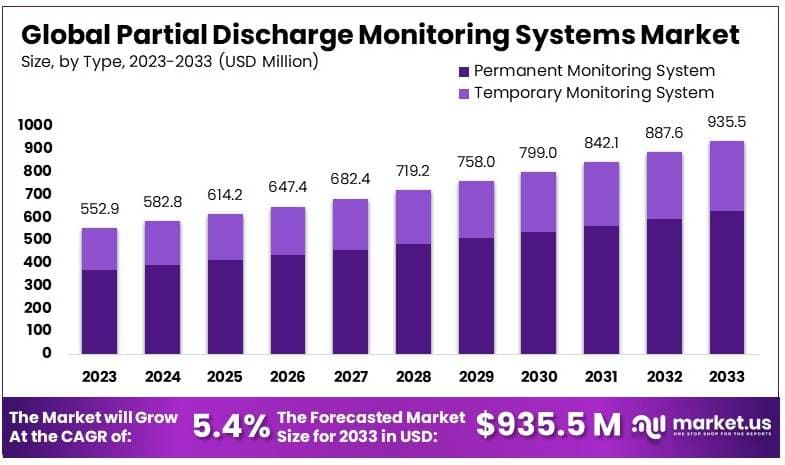
\includegraphics[width=0.7\textwidth]{graphic/MarketGrowth.png}
    \caption{Global Partial Discharge Monitoring Systems Market By Type (2023--2033), Showing Growth From USD~552.9~Million In 2023 To USD~935.5~Million By 2033 \parencite{Market.us._2024}.}
    \label{fig:market_growth}
\end{figure}

The global market for partial discharge monitoring systems is growing robustly, driven by the need for grid reliability and aging infrastructure. In 2023, the partial discharge monitoring market was valued around USD 550–580 million, and is projected to reach approximately USD 740–935 million over the next 5–10 years. This reflects a healthy compound annual growth rate on the order of 5–6\%. Investments in smart grids and preventive maintenance are key factors propelling this growth \parencite{Jia_2020, Kim_2020}. Notably, Asia Pacific is the leading region in partial discharge monitoring adoption, as countries like China, India, and Japan heavily invest in such systems to support their large power networks \parencite{Song_2018, Abdullah_2019}. North America and Europe also represent significant markets, with North America comprising roughly one-third of demand (about 35\% in 2023) amid major grid modernization efforts. Malaysia, as part of the dynamic Asia Pacific region, is seeing increased attention to partial discharge monitoring through its national utility initiatives, although its domestic market size is a modest portion of the global figure \parencite{Chan_2023}. The trend worldwide is clear: utilities and industries are allocating more budget to partial discharge detection technology as part of broader condition-based maintenance and grid reliability programs \parencite{Sikorski_2020}.

From an investment standpoint, global utilities and governments are channeling substantial funds into grid monitoring technologies, including partial discharge systems. For example, the European Union has mandated regular partial discharge assessments and earmarked about €200 million specifically for upgrading infrastructure with advanced partial discharge monitoring by 2025. In the United States, utilities invested roughly USD 168 billion into the electric grid in 2023, with about USD 30.7 billion directed to transmission and USD 57.1 billion to distribution upgrades. A portion of these investments goes toward installing sensors and online monitoring (such as partial discharge detectors) to preempt failures \parencite{Liccardo_2022}. Government-backed programs, such as the U.S.\ Department of Energy’s Grid Resilience and Innovation Partnerships, totaling USD~2.7~billion in funding, further illustrate the strong emphasis on modernizing grid monitoring and diagnostic capabilities. In Asia, state-owned utilities are adopting similar approaches for example, State Grid China has deployed innovative solutions, including UAV-based ultrasonic partial discharge detection systems, to patrol and maintain its extensive transmission network \parencite{Kim_2020}. Overall, both private-sector investments and public-sector funding mechanisms demonstrate a clear and sustained trend toward strengthening partial discharge monitoring as a core component of critical infrastructure development.

\subsection{Economic Impact of partial discharge-Related Outages and Failures}

Partial discharge is not just a technical issue; its consequences carry heavy financial costs. Partial discharge activity deteriorates insulation over time and is a leading cause of electrical equipment failures, which in turn can trigger power outages \parencite{Hussain_2021, Agarwal_2023}. Studies indicate that a substantial proportion of disruptive power apparatus failures—on the order of 80--85\% in high-voltage substations—are attributable to partial discharge activity \parencite{Sikorski_2020}. When such failures occur, the associated economic consequences can be severe, resulting in industrial downtime, revenue losses for utilities, and substantial recovery and repair costs. To put this in perspective, power outages cost businesses and economies billions annually. In the United States, for example, sudden power outages cost businesses over \$150 billion each year. In Malaysia, a single major blackout (the 2003 nationwide outage) was estimated to have cost local businesses about USD 13.8 million. 

Even smaller-scale partial discharge incidents can incur tens of thousands of dollars in losses per day for the affected facility. A case study from a wind farm showed that partial discharge-induced tripping of a circuit breaker caused over \$24,000 in lost revenue in just one occurrence. For utilities, a damaged transformer or switchgear that takes down a substation can mean costs reaching hundreds of thousands of dollars per day in unmet demand and repair efforts \parencite{Aslam_2022}. These direct costs are compounded by indirect losses: lost productivity, spoiled products, and cascading effects on other businesses and services. It's no surprise, then, that avoiding unplanned outages is a top financial priority for power providers and consumers alike. Beyond individual incidents, chronic reliability issues have macroeconomic impacts. Frequent outages erode investor confidence and can stunt economic growth. South Asian economies, for instance, have been shown to suffer substantial GDP deficits due to power supply disruptions. In the corporate world, downtime can affect everything from manufacturing output to data center operations and safety systems. U.S. industry experts argue that many outage cost estimates actually understate the true impact, since they often fail to capture follow-on losses across supply chains and society. In summary, partial discharge related failures impose substantial economic costs, thereby underscoring the importance of investing in partial discharge monitoring systems, as the cost of preventive measures is significantly lower than the cost associated with unanticipated equipment failure.


\subsection{Government Funding and Policies on partial discharge Monitoring Infrastructure}

Governments and regulators worldwide recognize the importance of grid reliability and have introduced policies and funding initiatives that, directly or indirectly, support partial discharge monitoring deployment.Malaysia’s government, through the Energy Commission (Suruhanjaya Tenaga) and regulatory frameworks such as Incentive-Based Regulation, has established system reliability as a key performance metric for electric utilities. Under the Incentive-Based Regulation framework, Tenaga Nasional Berhad—Malaysia’s primary electric utility—is incentivized to invest in infrastructure upgrades and preventive maintenance strategies aimed at minimizing supply interruptions. This policy approach has resulted in sustained investments in technologies such as online partial discharge detection systems, high-speed protection schemes, and systematic asset replacement programs to enhance grid resilience \parencite{Abdullah_2019}. The effectiveness of these measures is reflected in the System Average Interruption Duration Index for Peninsular Malaysia, which was recorded at only 48.13~minutes per customer in 2019, outperforming many developed economies. This level of reliability is attributed in part to the proactive identification and mitigation of incipient insulation faults, including partial discharge activity, before they escalate into major system failures. The Malaysian government also supports research and development in grid monitoring through agencies like Tenaga Nasional Berhad Research and various university grants, fostering local expertise in partial discharge detection techniques \parencite{Chan_2023}.

Elsewhere in Asia, governments are bolstering grid resilience which includes partial discharge monitoring as a component. China's government, via State Grid and Southern Grid, has poured funding into modernizing its vast transmission network – including installing continuous monitoring sensors and even using drones for partial discharge inspections \parencite{Kim_2020}. India has launched programs to upgrade its aging transmission and distribution infrastructure, backed by government financing and multilateral loans, which often stipulate the adoption of better monitoring to reduce technical losses and outages. Southeast Asian countries like Singapore and Thailand have also updated their grid codes and standards to encourage condition-based maintenance; utilities in these countries increasingly use partial discharge testing as part of equipment commissioning and routine checks \parencite{Wang_2024}. On the international stage, organizations such as the International Electrotechnical Commission have set standards (e.g. IEC 60270) that many governments adopt or reference, effectively making partial discharge measurement a normative requirement during factory testing and on-site commissioning of high-voltage equipment \parencite{Vera_2023_1}. Additionally, the World Bank and regional development banks fund electrification and grid reliability projects in developing nations, often including components for training and equipment to implement partial discharge monitoring as a means to extend asset life.

In advanced economies, regulatory pressure is perhaps most formalized in Europe and North America. Several European countries mandate periodic partial discharge testing for critical grid assets as part of their preventive maintenance regulations. The EU's focus on smart grids and its large funding programs (like the European Green Deal investments in energy networks) explicitly list grid diagnostic technologies eligible for support. In the United States, while no federal law specifically compels partial discharge monitoring, the trend is guided by reliability standards and incentives. The North American Electric Reliability Corporation has reliability standards that push utilities toward robust maintenance of key equipment (transformers, breakers, etc.), and partial discharge monitoring is recommended as a best practice in industry guidelines for preventing insulation failures \parencite{Hussain_2021}. U.S. federal funding through the Department of Energy's grid modernization initiatives and infrastructure bills has provided billions for grid upgrades, implicitly encouraging utilities to include advanced sensors (partial discharge, thermal, etc.) in their plans. In summary, government policies worldwide increasingly favor proactive maintenance and infrastructure resiliency, creating an environment where partial discharge monitoring is not just optional but often a supported or expected investment. This alignment of policy and funding with the goal of reducing blackouts has accelerated the adoption of partial discharge monitoring technology on a global scale.

\subsection{Industry Initiatives and partial discharge Monitoring Programs}

Electric utilities and industry players are at the forefront of implementing partial discharge monitoring as part of their asset management strategies. In Malaysia, both Tenaga Nasional Berhad and Sabah Electricity Sdn. Bhd. have launched initiatives to improve grid reliability that include partial discharge management. Tenaga Nasional Berhad, which serves Peninsular Malaysia, has been a regional leader in reliability and has systematically rolled out condition-based maintenance programs \parencite{Abdullah_2019}. As part of these efforts, Tenaga Nasional Berhad pioneered partial discharge mapping techniques on its medium-voltage cables, conducting extensive field trials as early as the 2000s to evaluate their effectiveness. Today, Tenaga Nasional Berhad employs online partial discharge detection systems and partial discharge mapping in its operations for example, to continuously monitor underground power cables and detect insulation defects before they escalate \parencite{Abdullah_2019}. According to Tenaga Nasional Berhad's recent reports, integrating partial discharge monitoring has been instrumental in early fault identification and has helped mitigate the likelihood of major failures in the distribution network. Tenaga Nasional Berhad has extended these predictive maintenance practices to critical equipment like 33 kV switchgears, again using partial discharge sensing to preempt flashovers and catastrophic breakdowns \parencite{Alsumaidaee_2022}. By catching warning signs like partial discharge, Tenaga Nasional Berhad can schedule maintenance or component replacements proactively, thereby keeping its System Average Interruption Duration Index and System Average Interruption Frequency Index indices at impressively low levels. This approach directly translates to fewer outages and improved service continuity for customers.

Sabah Electricity Sdn. Bhd., which manages the grid in Sabah, has also recognized the importance of such monitoring, albeit starting from a more challenging reliability baseline. Historically, Sabah experienced frequent power supply disruptions; in 2005, the System Average Interruption Duration Index exceeded 4{,}000~minutes per customer, reflecting a very low level of system reliability. Through various programs, Sabah Electricity Sdn. Bhd. has dramatically improved this, reducing System Average Interruption Duration Index to about 274 minutes in 2023 and setting a target of 100 minutes by 2030. To achieve this, Sabah Electricity Sdn. Bhd. is upgrading its infrastructure and maintenance regimes. While specific partial discharge monitoring programs at Sabah Electricity Sdn. Bhd. are less publicized than Tenaga Nasional Berhad's, the utility is known to be collaborating with Tenaga Nasional Berhad and technical partners to adopt similar best practices. This likely includes using portable partial discharge detection units for surveying substations and cables and prioritizing the replacement of equipment that shows partial discharge symptoms \parencite{Sikorski_2025}. The Malaysian government has been supportive, with federal funds aiding Sabah's grid improvements (including a subsidy to cover Sabah Electricity Sdn. Bhd.'s operational deficits while upgrades are underway). Industry-wide, there is also knowledge sharing: Tenaga Nasional Berhad Research and local universities have worked on partial discharge detection techniques suited for the tropical environment (where high humidity can exacerbate surface discharge) \parencite{Azam_2023}. These R&D outputs benefit Sabah Electricity Sdn. Bhd. and other regional utilities in crafting their partial discharge monitoring and mitigation strategies.

Beyond the utilities, industry involvement includes equipment manufacturers and service providers who run partial discharge monitoring programs or services. Companies like Doble, Megger, Qualitrol, and EA Technology offer partial discharge testing as part of substation maintenance contracts and have conducted training workshops in Malaysia and across Asia to build local capacity. Some large industrial consumers (e.g. semiconductor factories or oil & gas facilities in Malaysia) have also started installing partial discharge monitors on their critical high-voltage equipment to avoid costly downtime. For instance, continuous partial discharge monitoring systems are now available for large motors, generators, and gas-insulated switchgear and vendors often cite success stories where their systems gave early warnings that averted a failure \parencite{Seri_2021}. An example of such detection technology is illustrated in Figure~\ref{fig:fluke_camera}. Global industry statistics further underscore the value of partial discharge monitoring; one industry source reports that approximately 85\% of disruptive substation failures are attributable to partial discharge activity, indicating that the implementation of partial discharge monitoring programs can significantly reduce the risk of such failures \parencite{Sikorski_2020}. Another industry report highlighted that insulation failure (often traceable to partial discharge) contributes to up to 90\% of switchgear defects, reinforcing why so many maintenance teams now include partial discharge checks as a standard procedure \parencite{Alsumaidaee_2022}.

\begin{figure}[h]
    \centering
    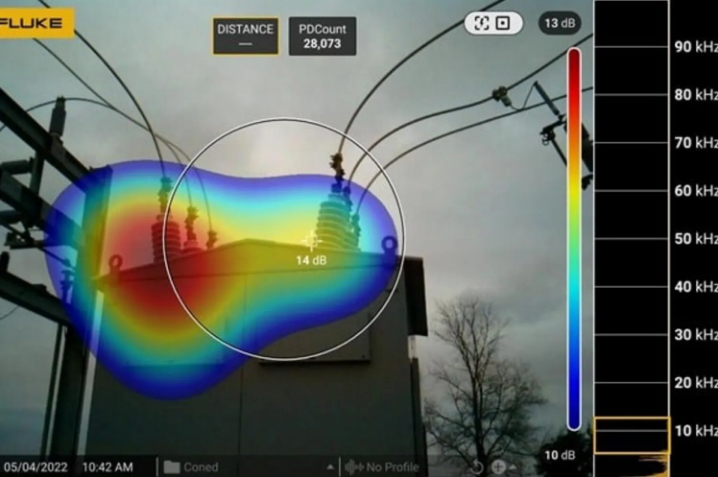
\includegraphics[width=0.7\textwidth]{graphic/FlukeCamera.png}
    \caption{Example of partial discharge detection using an acoustic imaging camera (Fluke ii910), where colored contours indicate partial discharge intensity on substation bushings. \parencite{Fluke_nd}}
    \label{fig:fluke_camera}
\end{figure}

In the Malaysian context, the collaboration between industry and the national utility is evident in programs like the Intelligent Predictive \& Diagnostic Monitoring system mentioned by Tenaga Nasional Berhad, which integrates partial discharge sensors in the broader smart grid monitoring platform. Tenaga Nasional Berhad and Sabah Electricity Sdn. Bhd. also participate in regional forums (through ASEAN utilities and international bodies) to share incident statistics and lessons. While detailed partial discharge incident statistics in Malaysia are not publicly released, anecdotal evidence and case reports suggest that numerous minor faults have been caught and resolved thanks to partial discharge detection, preventing them from becoming major outages. Each avoided incident contributes to improved reliability metrics. The drop in Tenaga Nasional Berhad's transmission system minutes (only 0.27 minutes of interruption in 2019 for Peninsular Malaysia) is partly credited to such preventive monitoring. Regionally, countries like Singapore report very low outage rates as well, attributable to stringent monitoring and maintenance regimens (which include partial discharge testing). This industry-wide push from utility engineers patrolling with ultrasonic partial discharge detectors, to control centers analyzing continuous online partial discharge data highlights a robust commitment to nipping problems in the bud \parencite{Abdullah_2019, Alshalawi_2024}.

\section{Existing Approaches and Challenges}

The diagnosis of partial discharge (PD) is a critical aspect of condition monitoring for high-voltage equipment, providing essential insights into the health of insulation systems \parencite{Hussain_2021}. Diagnostic approaches have evolved from traditional methods, which rely on the manual interpretation of discharge patterns, to modern automated systems employing artificial intelligence and machine learning \parencite{Masud_2016}. While conventional techniques have been foundational, they are often limited by subjectivity, inefficiency in handling large datasets, and susceptibility to noise, which can compromise diagnostic accuracy \parencite{Florkowski_2021, Das_2023}.

To address this issue, automated methods have been developed to provide more objective and efficient analysis \parencite{Lu_2020_2}. However, these advanced systems introduce their own set of challenges, including the complexity of robust feature extraction, the need for effective noise cancellation, and ensuring model generalization across varied operational conditions \parencite{Friebe_2024, Long_2024}.

\subsection{Limitations of Traditional Methods}
\label{sec:limitations_traditional}

Conventional methods for diagnosing partial discharge phenomena primarily rely on the manual interpretation of Phase-Resolved partial discharge patterns by skilled operators \parencite{Kasinathan_2017, Florkowski_2021}. This approach, while historically effective, is increasingly recognized for its inherent limitations, which hinder its applicability in modern high-voltage insulation systems.

One of the foremost challenges in manual partial discharge analysis is its subjectivity. The interpretation of Phase-Resolved partial discharge patterns depends heavily on the experience and expertise of the operator, making it susceptible to human error \parencite{Masud_2016, Lu_2020_2}. Variations in individual judgment can lead to inconsistencies in diagnosis, ultimately affecting the reliability of the results \parencite{Kunicki_2018}. Such subjectivity poses a significant risk in critical applications where precise partial discharge identification is essential for ensuring equipment longevity and operational safety.

Another major drawback is the time-consuming nature of manual partial discharge analysis. Evaluating large volumes of Phase-Resolved partial discharge data requires substantial effort and expertise, making the process inefficient, particularly for large-scale industrial applications \parencite{Long_2024}. As the demand for faster and more efficient partial discharge diagnosis grows, the reliance on human interpretation becomes increasingly impractical, emphasizing the need for automated techniques that can process large datasets more efficiently \parencite{Das_2023}.

Furthermore, traditional partial discharge diagnosis methods are highly susceptible to noise interference, which poses a significant challenge in real-world applications \parencite{Friebe_2024}. In practical scenarios, especially in on-site measurements, partial discharge signals are often masked by background noise, making it difficult to distinguish genuine partial discharge activity from external disturbances \parencite{Ghosh_2020, Bao_2024}. Conventional filtering techniques are not always effective in isolating partial discharge signals, leading to potential misclassification or overlooked defects \parencite{Hussein_2016}. The presence of noise-induced errors further complicates the reliability of manual Phase-Resolved partial discharge pattern interpretation.

In addition to noise susceptibility, conventional techniques struggle to handle complex partial discharge scenarios where multiple partial discharge sources coexist within an insulation system \parencite{Baug_2017}. In such cases, overlapping partial discharge patterns make it challenging to extract meaningful features and perform accurate classification \parencite{Biswas_2016, Firuzi_2017}. Traditional methods often lack the capability to effectively differentiate between multiple partial discharge sources, limiting their diagnostic accuracy and effectiveness. This limitation is particularly problematic in aging power equipment, where different types of insulation defects may simultaneously contribute to partial discharge activity.

\subsection{Challenges with Automated Methods}

Given these challenges discussed in Section~\ref{sec:limitations_traditional}, there is a growing need for advanced partial discharge diagnosis techniques that can overcome the limitations of manual interpretation. The integration of machine learning and signal processing methods has shown promising potential in addressing these issues by providing objective, efficient, and noise-resilient partial discharge classification \parencite{Masud_2016, Lu_2020_2}. These approaches offer significant advantages, including improved efficiency, objectivity, and the ability to process large volumes of data. However, despite their potential, automated methods still face several fundamental challenges that must be addressed to achieve reliable and accurate partial discharge classification.

One of the primary challenges in automated partial discharge classification is the process of feature extraction. Effective partial discharge analysis requires the selection of meaningful features that can accurately represent different types of discharge activity \parencite{Long_2024}. However, partial discharge signals are complex and often exhibit highly stochastic behavior, making it difficult to determine which features are most relevant for classification \parencite{Dai_2017}. The process of selecting and engineering features typically requires significant domain expertise to ensure that extracted parameters adequately capture the characteristics of different partial discharge types \parencite{Zhou_2017}. Without careful feature selection, machine learning models may struggle to distinguish between genuine partial discharge signals and external noise, leading to misclassification and unreliable diagnostic outcomes.

Another significant obstacle is the optimization of machine learning algorithms for partial discharge classification. Selecting the most suitable algorithm is not always straightforward, as different techniques exhibit varying levels of effectiveness depending on the nature of the partial discharge data \parencite{Fei_2024}. The stochastic nature of partial discharge signals further complicates this process, as the variability in signal characteristics makes it difficult to establish a universally optimal model \parencite{Vigneshwaran_2022}. Furthermore, machine learning algorithms often require fine-tuning of hyperparameters to achieve high classification accuracy. This optimization process can be computationally intensive and may necessitate extensive trial-and-error experimentation to identify the best-performing configurations.

Beyond algorithm selection and optimization, a major concern with automated partial discharge classification is the issue of generalization. Many machine learning models struggle to generalize well when applied to new or unseen data \parencite{Raymond_2022}. This problem is particularly pronounced when models are trained on limited or imbalanced datasets, where certain partial discharge types may be underrepresented \parencite{Tuyet-Doan_2021}. As a result, the trained models may exhibit high accuracy on the training data but fail to maintain their performance when applied to real-world scenarios. The challenge of generalization necessitates the use of robust data augmentation techniques, transfer learning, or adaptive learning mechanisms to improve model resilience across different operating conditions.

Additionally, the presence of environmental noise and interference remains a significant challenge for automated partial discharge classification systems \parencite{Azam_2023}. In practical applications, partial discharge signals are often contaminated by external noise sources, making it difficult to isolate and identify discharge patterns accurately \parencite{Friebe_2024}. The effectiveness of an automated classification system heavily depends on the robustness of its feature extraction and noise filtering techniques. Advanced signal processing methods, such as wavelet transforms, adaptive filtering, and deep learning-based denoising techniques, have been explored to mitigate the impact of noise \parencite{Abdullah_2019, Jin_2019}. However, ensuring the reliability of partial discharge classification in noisy environments remains an active area of research.

\section{Problem Formulation}

\subsection{Research Gap}

Current research in partial discharge detection for overhead power lines often focuses on specific datasets or individual algorithms, lacking a comprehensive comparison of traditional and modern machine learning techniques across diverse datasets \parencite{Basharan_2018, Song_2018}. This limitation restricts the understanding of the relative strengths and weaknesses of different algorithms under varying conditions, such as noise levels, environmental factors, and signal acquisition setups. Performance reported on a single dataset may not generalize well to other datasets due to differences in partial discharge signal characteristics, noise profiles, and measurement protocols, necessitating a broader comparison across multiple datasets to assess the robustness and generalizability of different machine learning techniques. The optimal selection and combination of features for partial discharge detection also remain underexplored, with existing studies rarely investigating the impact of different feature sets, such as time-domain, frequency-domain, and deep-learned embeddings, on the performance of various machine learning models \parencite{Long_2024}. Different algorithms may be sensitive to specific feature types, and optimizing feature selection can significantly enhance detection accuracy and efficiency, making a systematic investigation of feature combinations crucial for identifying the most informative and discriminative features for each algorithm. This gap hinders the development of robust and generalizable partial discharge detection systems that can perform reliably across diverse overhead power line configurations and environmental conditions, and the lack of comprehensive algorithm comparisons and feature analyses makes it challenging to select the most appropriate algorithm and feature set for specific applications. This study aims to address this gap by providing a comparative analysis of traditional and modern machine learning methods across multiple datasets and investigating the impact of different feature combinations on their performance.

\subsection{Problem Statement}

Based on the identified research gap, this study addresses several key problems. First, there is a lack of a comprehensive comparison of machine learning algorithms for partial discharge detection, which includes evaluating the performance of traditional algorithms (Support Vector Machine, Random Forest, K-Nearest Neighbors, Naive Bayes, AdaBoost) in terms of accuracy, precision, recall, F1-score, Area Under the Curve, and computational cost, as well as understanding the trade-offs between performance and computational complexity, which is critical for real-time partial discharge monitoring in overhead power lines \parencite{Lu_2020_2, Kumar_2024_5}. Second, there is limited understanding of the optimal feature sets for different machine learning algorithms in partial discharge detection, requiring an investigation of various feature extraction techniques, including time-domain features (e.g., pulse amplitude, width), frequency-domain features (e.g., Fast Fourier Transform, wavelet transforms), and deep-learned embeddings, to evaluate their impact on the performance of each algorithm and identify the most discriminative features that contribute significantly to accurate partial discharge classification \parencite{Long_2024}. Third, there is a need to evaluate the generalizability of partial discharge detection models across diverse datasets, which involves testing trained models on datasets not used during training, representing different noise conditions, environmental factors, and signal acquisition protocols, to provide insights into the robustness and real-world applicability of the developed models for overhead power line monitoring \parencite{Raymond_2022}.

\section{Study Objectives}

Based on the hypotheses, this study aims to achieve the following objectives:
\begin{itemize}
    \item To identify the optimal feature set for each machine learning algorithm by evaluating different feature combinations.
    \item To compare the performance of various traditional machine learning algorithms (Support Vector Machine, Decision Tree, Random Forest, K-Nearest Neighbors, ANN) for partial discharge detection.
\end{itemize}

\section{Scope Of Work}

The scope of this thesis includes:
\begin{itemize}
    \item Preprocessing and feature extraction from publicly available partial discharge datasets. This involves applying signal conditioning techniques to remove noise and irrelevant components, followed by the extraction of features such as wavelet coefficients, phase-resolved partial discharge patterns, statistical descriptors, and entropy measures. Feature selection will be guided by existing literature and optimized to capture the characteristics of partial discharge activity under different conditions.
    \item Training and evaluation of traditional machine learning models using cross-validation on individual datasets and a combined dataset. This includes training each selected machine learning algorithm on individual partial discharge datasets using k-fold cross-validation to ensure statistical robustness. The trained models will then be evaluated on separate test sets as well as on the aggregated dataset to measure generalization performance.
    \item Comparison of model performance based on accuracy, precision, recall, F1-score, and computational time. These performance metrics will allow for a comprehensive evaluation of each algorithm, accounting for both predictive quality and computational efficiency, which are critical factors in practical deployment.
    \item Analysis of the impact of different feature combinations on the performance of each model. This involves systematic evaluation of various feature subsets and quantifying their influence on the classification results. The goal is to identify optimal feature sets that maximize detection accuracy while minimizing computational costs, thus supporting real-time monitoring applications.
\end{itemize}

\section{Organisation Of Thesis}

This thesis is organized as follows: Chapter 1 introduces the background, motivation, problem statement, hypotheses, objectives, and scope of the research. It provides a comprehensive overview of the context, rationale, and goals of the study, setting the stage for the subsequent chapters.

Chapter 2 reviews the existing literature on partial discharge detection, covering various methods and challenges. This chapter provides a detailed analysis of prior research in partial discharge analysis, including traditional machine learning techniques, signal processing approaches, and recent developments in automated diagnostics. It identifies current gaps and motivates the research direction of this study.

Chapter 3 details the methodology employed, including dataset acquisition, signal preprocessing, feature extraction, model selection, and performance evaluation. This chapter outlines the entire experimental pipeline, ensuring clarity and reproducibility. It describes the datasets used, the preprocessing strategies applied, the features extracted from partial discharge signals, and the machine learning algorithms selected for evaluation.

Chapter 4 presents the experimental results, comparing the performance of various machine learning algorithms and analyzing the effects of feature selection. This chapter includes comparative results across multiple datasets, evaluates generalization, and interprets model behavior in relation to feature sets.

Chapter 5 concludes the study by summarizing the key findings, discussing their implications for real-world partial discharge monitoring, and suggesting directions for future research. It highlights the contributions of the work and outlines opportunities to extend the study, such as integration with Internet of Things sensors or hybrid deep learning models.

The Appendix includes supplementary materials such as dataset details, signal transformation formulas, algorithmic configurations, and extended experimental results. This section serves as a technical reference for readers and researchers interested in replicating or building upon this work.
